\documentclass{article}
\usepackage[utf8]{inputenc}
\usepackage[margin=1.2in]{geometry}
\usepackage{hyperref}

\PassOptionsToPackage{usenames,dvipsnames,svgnames}{xcolor}  
\usepackage{tikz}
\usetikzlibrary{arrows,positioning,automata}

\usepackage{natbib}
\usepackage{graphicx}
\usepackage{amsmath}
\usepackage{listings}
\usepackage{xcolor}


\definecolor{codegreen}{rgb}{0,0.6,0}
\definecolor{codegray}{rgb}{0.5,0.5,0.5}
\definecolor{codepurple}{rgb}{0.58,0,0.82}
\definecolor{backcolour}{rgb}{0.95,0.95,0.92}
\definecolor{deepblue}{rgb}{0,0,0.5}
\definecolor{deepred}{rgb}{0.6,0,0}
\definecolor{deepgreen}{rgb}{0,0.5,0}

\lstdefinestyle{mystyle}{
    backgroundcolor=\color{white},   
    commentstyle=\color{codegreen},
    keywordstyle=\color{deepblue},
    numberstyle=\tiny\color{codegray},
    stringstyle=\color{deepgreen},
    emph={Agent,__init__,act,self,union,exists, scope},
    emphstyle=\color{deepred},
    basicstyle=\ttfamily\footnotesize,
    breakatwhitespace=false,         
    breaklines=true,                 
    captionpos=b,                    
    keepspaces=true,                 
    numbers=left,                    
    numbersep=5pt,                  
    showspaces=false,                
    showstringspaces=false,
    showtabs=false,                  
    tabsize=3
}

\lstset{style=mystyle}

\title{\vspace{-2 cm} Universidade Federal de Ouro Preto \\ BCC 325 - Inteligência Artificial \\ Prova 3}
\date{}


\begin{document}

\maketitle

\vspace{-2 cm}
\begin{enumerate}

\item (1 pt) Que tipo de problema resolvemos com o algoritmo de busca em profundidade? Quais dificuldades este algoritmo pode encontrar?

\item (1 pt) Que tipo de problema resolvemos com o algoritmo $A^*$? Qual a complexidade de tempo e espaço deste algoritmo?

\item (1 pt) Para o que serve um algoritmo de busca local?

\item (1 pt) Quais são os componentes de um problema de satisfação de restrições?

\item (1 pt) Como podemos utilizar busca local para resolver um problema de satisfação de restrições?

\item (1 pt) Considere os dados representados na figura abaixo. O que pode ser feito para que este problema seja resolvível com regressão logística?

    \begin{figure}[!ht]
        \centering
        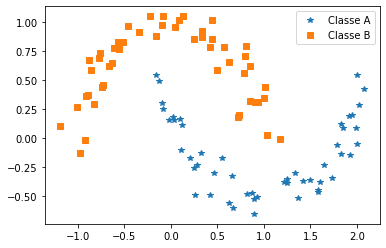
\includegraphics[width=0.41\textwidth]{moons.png}
    \end{figure}

\item (1 pt) Para o que serve o algoritmo de backpropagation? Como ele influencia a escolha das funções de ativação e de custo (perda) de uma rede neural artificial?

\item (1 pt) O que é overfitting? Quais são os indícios de que um modelo está sofrendo de overfitting? De forma geral, o que deve ser feito para diminuir o overfitting?

\item Considere a seguinte base de conhecimento (KB):
\vspace{-0.5 cm}

\begin{center}
    \begin{align*}
     a & \leftarrow b \wedge c. \\ 
     b & \leftarrow e. \\ 
     b & \leftarrow d. \\ 
     c &. \\ 
     d & \leftarrow h. \\ 
     e &. \\
     g & \leftarrow a \wedge b  \wedge e. \\
     f & \leftarrow h \wedge b. \\  
    \end{align*}
\end{center}


\begin{enumerate}
    \item (0.5 pt) Apresente um modelo da base de conhecimento apresentada.
    \item (0.5 pt) Apresente uma interpretação que não é um modelo da base de conhecimento apresentada.
    \item (0.5 pt) Mostre um prova bottom-up para esta base de conhecimento. 
    \item (0.5 pt) Apresente uma prova top-down para a pergunta $ask$ $g$.
\end{enumerate}

\end{enumerate}

\end{document}

